\chapter{Parametric Tensor Core Unit Architecture}
\label{ch}

\section{Chapter Overview}

The previous chapter introduced the parametric DPU in great details in regards to its implementation. As it has been studied, the constructed parametric DPU computes one dot product operation involving two vectors of four elements each plus an accumulation term. In this chapter, the scope moves one level higher: the goal is to show the design involved in constructing the parametric Tensor Core Unit which uses in its architecture the already described DPU. In fact, the TCU is not just one arithmetic block, but an organized architecture around several DPUs.

The method of RTL design of this upper level unit was built from a bottom-up approach. Several parametric DPUs are grouped inside an octet core. An octet core contains local buffers and the DPU array consisting of the parametric DPUs discussed in the previous chapter. Taking inspiration from NVIDIA, is also known that two octect cores are used inside the TCU datapath. Lastly, a finite state machine has also been designed to control the execution related to the TCU's datapath. 

So this chapter first explains the design objective. Then it introduces the thread-aware execution model. Afterwards it presents the top-level TCU architecture of the first release of designed in the thesis. It also shows the design of the execution related finite state machine. It also describes the datapath organization which will be explained to have the dual-octect structure, buffers and DPU arrays. The chapter also shows how format and width selections are propagated and finally it sumarizes the verification approach related to this unit. This chapter therefore acts as the bridge between the parametric DPU of chapter 3 and the integration work discussed in the following chapters.

\section{Design Objective and Architectural Approach}

As said, the parametric TCU was developed to move from one DPU to larger structure using more then one DPU for treating a larger oriented matrix block. The goal is not only arithmetic hence, but it regards that of organizing several dot-product operations. The TCU in fact is the architectural component which is the layer between the DPU which has been discussed before and the later level involving the processor/GPU integration described in the following chapters of this document.

The goal of the TCU, similarly to the DPU, is to be designed so that it supports more than one number format. This is implictly done already as the unit makes use of the DPU which already supports this. Consequently it is easy to understand that the arithmatic behavior of the TCU changes depending on the selected format/widht just like explained when introducing the parametric DPU.

Finally , from an architectural point of view, the roles of each component forming the TCU are well seperated. This is easily understood as the DPU handles the arithmetic computation specifically. The internal Buffers serve to handle operand staging for reuse mechanisms during the execution. The finite state machine on the other hand serves to handle sequencing. Overall, the datapath of the TCU handles parallel DPU execution. Thanks to this introduced property, it is easier to integrate the design to the modules like GPUs and this will be seen in the later integration related chapters. The next sections remind of the execution model, the top-level wrapper, the finite state machine and datapath and format selection.

\section{Thread-Aware Execution Model}

%paragraph 1: why the thread-awareness matters

The TCU involves operations which are cooperative with each other.  In general the matrix fregments are distributed and organized across multiple threads. Specifically, the concept is that the related hardware is organized considering a groups of threads. This motivates a thread-aware architecture instead of simple standalone arithmetic block \cite{raihan2019modeling}.

%paragraph 2: ThreadGroups and octets Define only what i need. 

Going to more detail, a threadgroup is defined as a group of four threads. In the designed TCU hardware, it is taken into inspiration the fact that two threadgroups cooperate. This specific group of hence eight threads is interprated as an octet. The octet becomes useful because it rapresents a natural unit for feeding part of the tensor core datapath. Also, the octet abstraction has been used conviniently to organize the datapath around groups of eight cooperating lanes. 

%paragraph 3: How this maps to the TCU

In the design of the TCU, the thread-aware idea was very usefull for design inspiration. In fact, it maps to the octect core. One octect core of the TCU corresponds to eight execution lanes / eight threads. The eight lanes are internally divided into two groups of four. Also the scope of the octect core in the design has the scope of the buffers. This means that in the implemented RTL design, the octect core inside the TCU has its own dedicated buffers along with its associated needed DPU array. The purpose is to stage operands and feed multiple parametric DPUs.

%paragraph4 : scope and transition 

This execution model involving the introduced concepts of threadgroups and octects provide the motivation of why it was convinient to build an octet-based design. Essentially, to make the software to hardware map more closer with each other. The following sections describe how this organization has been implemented in the RTL with more focus. First the top level wrapper is introduced and following will be introduced the control finite state machine and the datapath organization descriptions. 

\section{Top-Level Tensor Core Architecture}

The top level TCU is the highest hierarchical component of the overall TCU containing the datapaths as well as the control finite state machine. Externally, it is seen as the whole accelerator block receiving operands and control signals from the outside when it is to be integrated to GPUs or CPUs. The output of its signals are both in terms of control to signal the fact for instance that it is executing, as well as ones related to the data containing the result. The internal complexity of the components is hidden inside this wrapper unit. 

As explained, the wrapper is divided into control path and datapath. the control path is the finite state machine (also referred to as FSM). While the datapath is the computation and operand movement related to the MMA execution. At high level, the datapath consists of two octet cores. And each of these octet core contains buffers and DPU array.  A very high level block diagram initial view of the TCU can hence be visualized in Figure~\ref{fig:tcu_high_level} where the highest level components are observed inside the TCU wrapper.

This organization is the best because it separates nicely the control and datapath and consequently makes the design of the TCU much cleaner and understandable in relation to the threads executing it. It will be seen in more detail in the following sections that the FSM has the duty of deciding the sequence of operations related to a single HMMA instruction to execute on the TCU. While the datapath is the one which performs the staging and the computation itself leading to the final results of the accelerator. The next sections will describe the FSM and the datapath in a much more detailed point of view. 

\begin{figure}[htbp]
\centering
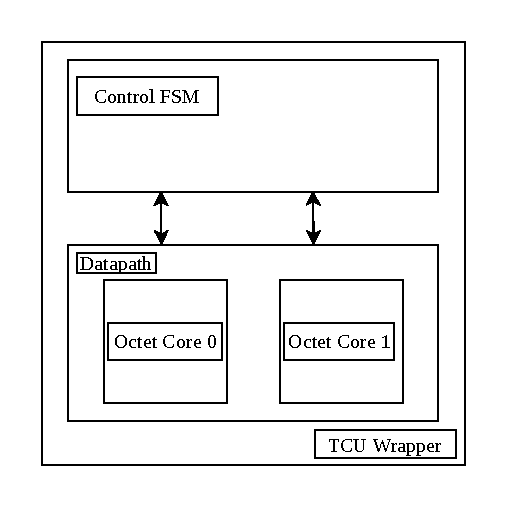
\includegraphics[width=1\textwidth]{Figures/highLevelTCU.pdf}
\caption{High-level organization of the Tensor Core Unit wrapper.}
\label{fig:tcu_high_level}
\end{figure}

\newpage
\section{Control Finite State Machine}

%goal is to introduce the FSM. why it is needed because the TCU operation happens in phases, not all at once.
%idea: fsm is the sequential logic, the datapath is the computational/storage logic.

The parametric TCU that is needed for the matrix workloads cannot do the whole related operation in one single uncontrolled step. In fact, the TCU's execution is performed in an organized matter through a control circuit which consists of a finite state machine guiding the TCU through its HMMA instruction execution. Inspiring from the TCU found in NVIDIA's GPUs, the operands which are related to the matrix multiply and accumulation operations must first load the operands first from their related register files of the threads into the tensor buffers. So, when an HMMA instruction is recognized, the operands must be loaded from the register files of the threads into related buffers.

More specifically, the different operands are loaded in different phases. There is a state dedicated to the fetching of the operands which are related to the A matrix from the register files. In that state, each of the threads which is performing the TCU operation loads into the buffers the associated registers which contain matrix A elements only. Analogously there are also dedicated states for the loading operations of the operands related to the B and C matrices into the related storage buffer elements. Importantly, for the states related to the loading of matrix A , B and C's operands, there are two states for each phase. This is because in the case the operands of the matrices are of 32 bit width, due to the construction of the TCU's buffers which will be introduced later, and due to the limited amount of ports of the register files related to the threads, there need to be two dedicated clock cycles for fetching the four 32 bit elements of a determined operand matrix. Said equivalently, if the load related to the four elements of an operand matrix is within 64 bits in total, then it is possible to fetch the four elements related to a specific matrix in a single clock cycle. Otherwise, the four elements associated to one HMMA instruction can be loaded in the related buffers in two clock cycles, corresponding to traveling in two load states of the FSM instead of one for a specific operand matrix. 

Another design decision of the controller FSM was related to the distinction of the HMMA instruction. In fact HMMA instructions which can execute on the TCU accelerator can be of either'step0' type, or of 'step1' type. If the HMMA instruction is of type step0, then each thread will load the 4 by 4 elements of A, of B and of C related to the operation. Else, if it is of step1 type, the threads need only to load new elements related to the matrix C, as the step1 instructions involve the multiplication of elements of A and B matrices which were loaded by other threads of the same octet which are hence already found in related octet buffers.  

After the loading related steps into the buffers, the datapath executes multiple computation steps which is done through the parametric DPUs. Specifically, in each of the execution steps of the FSM, four parametric DPUs associated to a threadgroup of the octet compute four outputs which correspond to a one by four intermediate result vector of the full four by four final result related to the HMMA instruction. Hence, there need to be in total four states of the FSM to produce the four by four intermediate result matrix associated to the HMMA instruction of a specific thread group. 

Lasty, Figure~\ref{fig:fsm_TCU} shows the concepts of the FSM circuit through the state diagram depiction, showcasing the states described previously and the flow of operations of the HMMA instruction executed on the TCU accelerator. 

\begin{figure}[htbp]
\centering
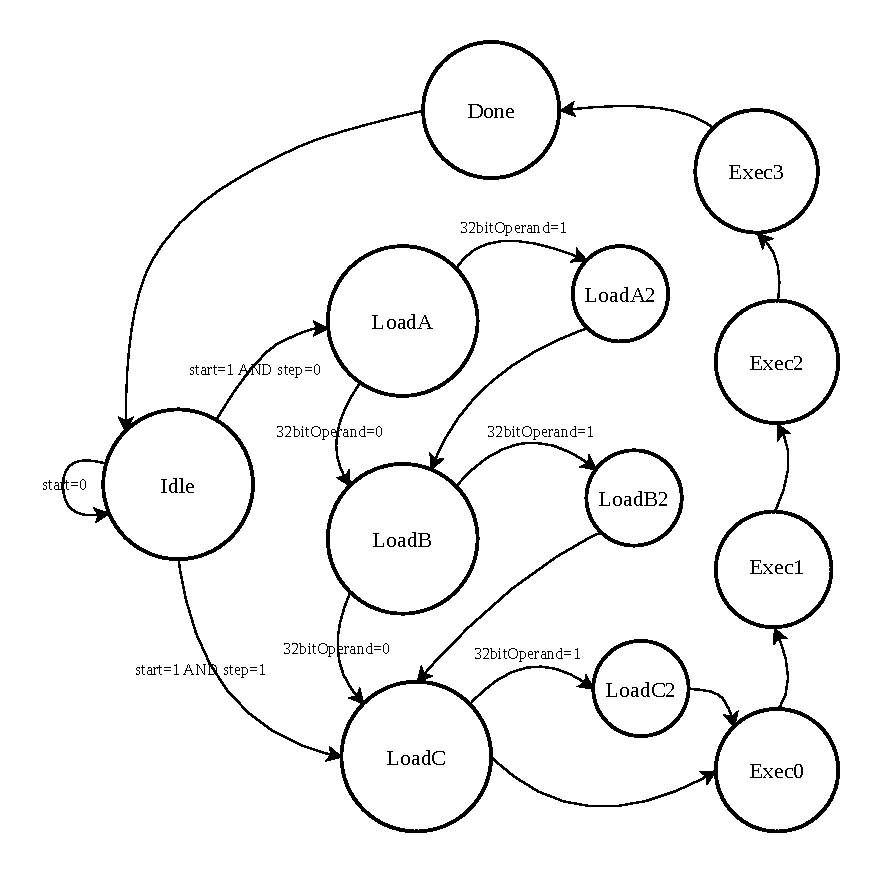
\includegraphics[width=1\textwidth]{Figures/FSM_TCU.pdf}
\caption{First Release of the FSM State Diagram Controlling the TCU's Datapath .}
\label{fig:fsm_TCU}
\end{figure}

\section{Datapath Organization}

%after explaining the control part in the previous section by explaining the fsm, we move to the part related to the computation.
After having explained the FSM circuitry associated to the TCU, which is part of the control related circuitry of the accelerator, it is important to remark the computation related elements composing the TCU. As explained, the FSM decides the sequence of inner steps performed in the related execution of an HMMA instruction done by the threads, while the datapath contains only the hardware descriptions which store the operands related to the singular HMMA instruction and executes the dot products of the MMA operation. As introduced previously, the main organization of the datapath is done by splitting the TCU into two octet cores. Each octet core is associated to two thread groups meaning eight threads in charge of the operability of this inner unit. 

Regarding the components embedded inside an octet core, each octet core contains two general elements: the octet buffers and a parametric DPU array. Both will be analyzed more in detail in this section. The datapath of the TCU in general receives control signals from the FSM and is able to understand on the basis of those signals when to activate the units composing the octet core in order to carry the computation related to the HMMA instruction at hand. Importantly, the datapath propagates related intermediate results and status signals back toward the higher level wrapper TCU unit in order so that eventually they may be  placed inside the related destination registers of the register files. 

\subsection{Dual-Octet Core Structure}

%what is the meaning of organizing the datapath as two octet cores ? ... architectural resons... 
%paragraph1: position in the hiererchy.
Earlier in this document, the top level TCU wrapper has been introduced as an organization of datapath and controller. The datapath part of such organization regarding this implementation can be considered to be non monolithc as it is divided into two symmetric octet core unit components. Each octect core is an intermediate block between the full TCU and the DPU arrays and this is the proof of an hiererchical design.

%paragraph2: meaning of one octect core.
One octet core component specifically groups local computation resources which are shared across two thread groups of four threads each. In fact, in one octet core the values fetched between the two threadgroups composing the octet are shared among them, allowing to efficiently perform the computation by exploiting reusaiblity of associated operands. Therefore this allows to make the overall TCU operation (which is a set of HMMA instructions) to be more efficient since the HMMA instructions related to the 'step1' type previously described have to load less elements into their buffers. This is because certain elements have been already loaded by the threads belonging to a different threadgroup but still related to the same octet. 

The overall high level diagram of the one octet core unit is found in figure Figure~\ref{fig:octetCore}. It shows the buffers associated to the octet of threads which are to utilize such hardware in execution. Specifically, the figure is related to the octet 0 which is the one composed of thred groups 0 and 4. The four threads in thread group 0 utilize lanes 0 to 3 depicted in the picture for loading the related A0, B0, and C0 buffers related to the matrix elements which they are in charge of. While on the other hand, the treads associated to thread group 4 utilize lanes 16 through 19 of the hardware, filling the buffers A1, B1, and C1. In the diagragram it can be noticed that thanks to the buffers, threads can utilize the values loaded by the threads of the opposite thread group of the same octet so that reusability is exploited and efficiency is increased. More details regarding the inner components depicted inside the octet core will be given in the following subsections. 

%paragraph3: why two octet cores
The reason why there are two octet cores is for the increasing of parallelism of the overall accelerator. Also two octet cores keep the datapath symmetric and avoids one large monolithic compuatation block design. Both the cores can be driven by one common control logic. Lastly, two octet cores makes the architecture easier to scale test and also to explain as the mapping of software to hardware is easier to depict.  

\begin{figure}[htbp]
\centering
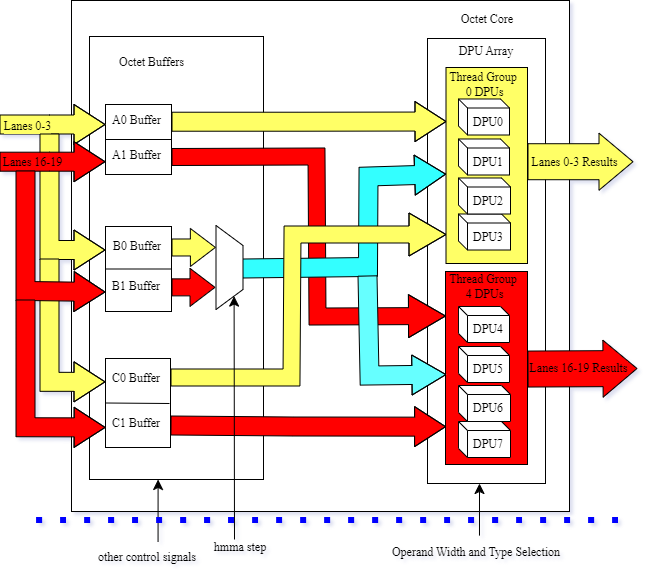
\includegraphics[width=1\textwidth]{Figures/octetCoreRel0.png}
\caption{First Release of the octet Core Datapath Containing the Octet Buffers and the DPU Array Embedded Elements.}
\label{fig:octetCore}
\end{figure}

\newpage
\subsection{Octet Buffers and Operand Staging}

%okay so this section right here will answer... how are operands prepared before the DPU array computes ? 

%paragraph 1: why are buffers needed ?
The buffers are needed for the operand staging fetched from the register files to be utilized in the tensor core's dot product operations. They help because they provide a cleaner execution flow, as well as giving the availability for the threads to utilize operands which were loaded by other threads not belonging to the same thread group of the octet. 

%paragraph 2: what is staged ? 

Buffers related to the octet stage the operands related to 4 by 4 matrix fragments related to the intermediate result calculation of a 4 row by 8 column matrix result. The buffers labeled as A and B in figure are the fragmanents related to matrices A and B while C is the accumulation buffer storing matrix C fragment if the given HMMA instruction belongs to the first set, else it stores the intermediate results needed for accumulation leading to the final result. 

%paragraph 3: FSM control of buffers

To understand which operation to be done by the buffers between loading, or giving the results to the DPU array to execute, the control signal of the FSM are interfaced to the octet buffers. There is a load enable signal which enables the loads synchronously. There is also a specific control signal which selects which kind of buffer needs to be loaded depending on the current state of the FSM, the load phase signal. Additionally, there is the load pair signal for making the buffers execute the loading phase longer in the case the specific format used has operands of 32 bit width. Lastly, as said previously there is the control signal related to making the buffer understnad whether the present HMMA instruction is of step 0 or step 1 type. This last distinguishment is necessary because between step0 and step 1 the four by four HMMA matrix fragment of B utilized for the computation changes in bulk. A detailed rapresentation of the first release of a singular octet buffer is shown in the Figure ~\ref{fig:octetBuffers}. the figure is related to octet 0 again as it mentions lanes 0 to 3 which are ran by the threads of thread group 0 and lanes 16 to 19 which are dedicated to the elements related to thread group 4. Lastly, each of the entries of the buffers loaded by either thread groups stores a one by four vector of a related 4 by 4 matrix fragment.


\begin{figure}[htbp]
\centering
\includegraphics[width=1\textwidth]{Figures/octetBuffer.png}
\caption{First Release of the octet Core Buffers Used For Operand Staging For the DPU Array Execution.}
\label{fig:octetBuffers}
\end{figure}

\newpage
\subsection{Parametric DPU Array}

% trying to answer how are buffered operands actually computed?

In the octet core, after the operands are staged in the buffers they are sent to the computation units which are collected in the DPU array circuit. The DPU array as the name suggests is a collection of parametric DPU units receiving their operands from the buffers. Each DPU of the array performs the dot-product primitive introduced in chapter 3.

Inside the DPU Array there are in total eight DPUs. This means that in parallel, the threads are able to execute eight dot product operations. More in detail, the DPU array of a single octet core outputs two 1 by 4 intermediate resulting vectors which will eventually be staged inside the register files. Considering that the FSM has four execution related states, and considering that the octet core is being executed by two threadgroups in parallel, then in the span of the four FSM execution states two 4 by 4 HMMA result fragments are being computed by the singular octect core.

The DPU array reuses the parametric DPU architecture introduced in chapter 3. For this reason, format and width selection are not redefined at the TCU level. The same selection signals are propagated to the instantiated DPUs, allowing the overall TCU structure to remain unchanged while only the arithmetic behavior inside each DPU changes according to the selected numerical configuration.


From a design point of view, the DPU array related to the octet core is responsible for computing a 4 by 4 intermediate result fragment of the HMMA instruction for each thread group. but since the DPU Array of the octect output two 1x4 vector results per time, there need to be three additional execution steps to give off the remaining six vectors needed for the result of the related HMMA instruction related to the thread groups of the octet. Because of this reason, there are buffers at the output of the array which collect the 1by4 vectors computed by the dpus. This way when the FSM enters a new execution step to calculate a new intermediate resulting 1 by 4 vector contributing to the HMMA fragment result, the previously calculated vector wont be lost. This and the overall DPU array described in this section is shown in the detailed Figure ~\ref{fig:octetDPUArray}. Specifically, the Figure shows the execution when the FSM is in the first of the four execution states the 'exec0' state. The bottom of the figure highlights the overall operation which is being xecuted in the exec0 state by the two threadgroups, as well as the high-level components embedded in one octet DPU array module. 

\begin{figure}[htbp]
\centering
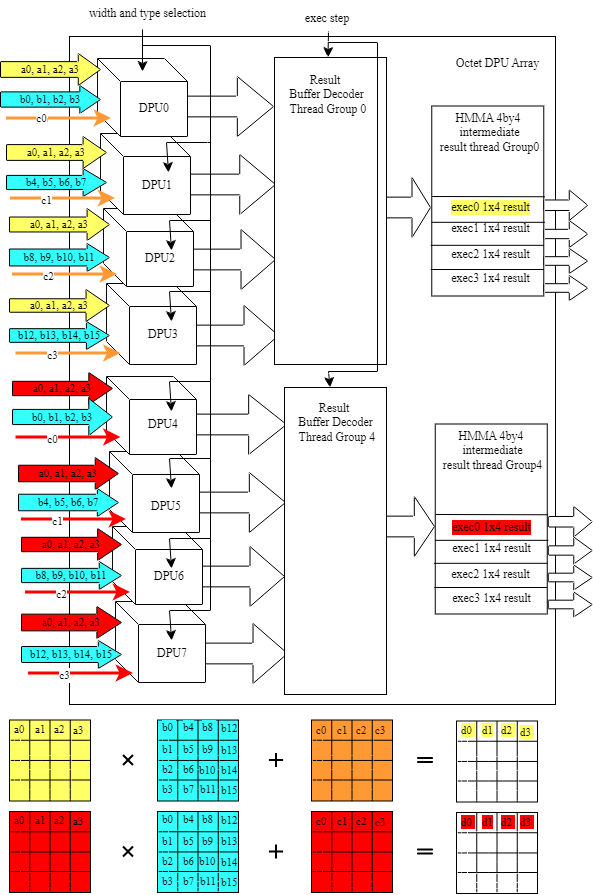
\includegraphics[width=1\textwidth]{Figures/octectDPUArray.png}
\caption{First Release of the octet Core DPU Array and elements involved in the HMMA instruction operation during the 'exec0' FSM state.}
\label{fig:octetDPUArray}
\end{figure}

\newpage
\section{TCU Functional Verification}

%section needed to try and answer: does the standalone TCU execute the intended sequence correctly ? . the goal of this section is to show that the standalone TCU works correctly in simulation.

%paragraph1: the purpose of the verification
The TCU described in the previous sections of this chapter has also been verified through simulation. The overall goal of this step was to check the correct sequence of the standalone TCU. Particularly in checking the correct sequencing of the signals belonging to the FSM and DPU arrays of the octets. The TCU involves two octet core units and hence the verification involves also the correctness of such units implicetly as well. The verification of the standalone TCU accelerator is done at the RTL level simulation level with the Vivado tool.

%paragraph 2: Testbench setup.

For verifying this first release of the parametric TCU, several steps of a general flow have been made. The first step was that of making a python script which was able to produce pseudo-random 16 by 16 A, B and C matrices relating to a multiply accumulation operation which involves four sets of HMMA step 0 and step 1 instructions specifically related to a target format. The python script script outputs the encoded and decoded values of the operands. It also calculates the most accurate decoded and encoded result matrix specific to the test. This first script also produces an input file for the testbench which bacicly gives the elements of the operand matrices so that the buffers are able to obtain the inputs for the tests. Lastly, after the simulation is done, the related RTL-testbench saves the intermediate results of the singular HMMA instructions and most importantly it saves the final 16 by 16 matrix which was obtained by the TCU simulation. Another python script takes this output simulated result and calculates the error with respect to the golden matrix which has been produced by the first script introduced in this flow. 

%paragraph 3: observed simulation behavior. 

To check the correct opration of the implemented inner components of the TCU analyzed in this section, initially the simulation waveforms of Vivado have been observed. After the start is asserted, the FSM follows the expected sequence of operation related specifically to the numerical format which is being tested. More specifically, it was checked if the loading states made the buffers of the accelerators be filled with the values rapresenting the operands. As well as checking if the execution steps happened like intended. Lastly, it was checked visually if the done signal was asserted correctly indicating the end operation of a related HMMA instruction.

%paragraph 4: waveform reference.

An example waveform regarding the simulation of one HMMA step 0 instruction targeting an innter test regarding posit 16 format operands is portrayed inf Figure Figure~\ref{fig:tcu_functional_waveform}. As it can be seen, it portrays the correct flow of the FSM idle, loading, execution and completion related control states. It also presents the content of the octet buffers for the operand matrices being updated in the proper timing, as well as the TCU's signals related to the results for this singular HMMA instruction.

%paragraph 5: 

The waveforms observed in Vivado were particularly useful for debugging the TCU's RTL descriptions if the results of the last HMMA instruction of the full set were different then the expected ones of the final matrix. 


Lastly, it is important to remark that the verification explained in this section only applies to standalone functional RTL behavior. It does not evaluate the area and timing of the associated RTL modules, nor presents the metrics related to the performance and the error of the operations. These specific reults regarding each specific format DPUs embedded inside the TCU will presented in the later chapters of this work. 

\begin{figure}[p]
\centering
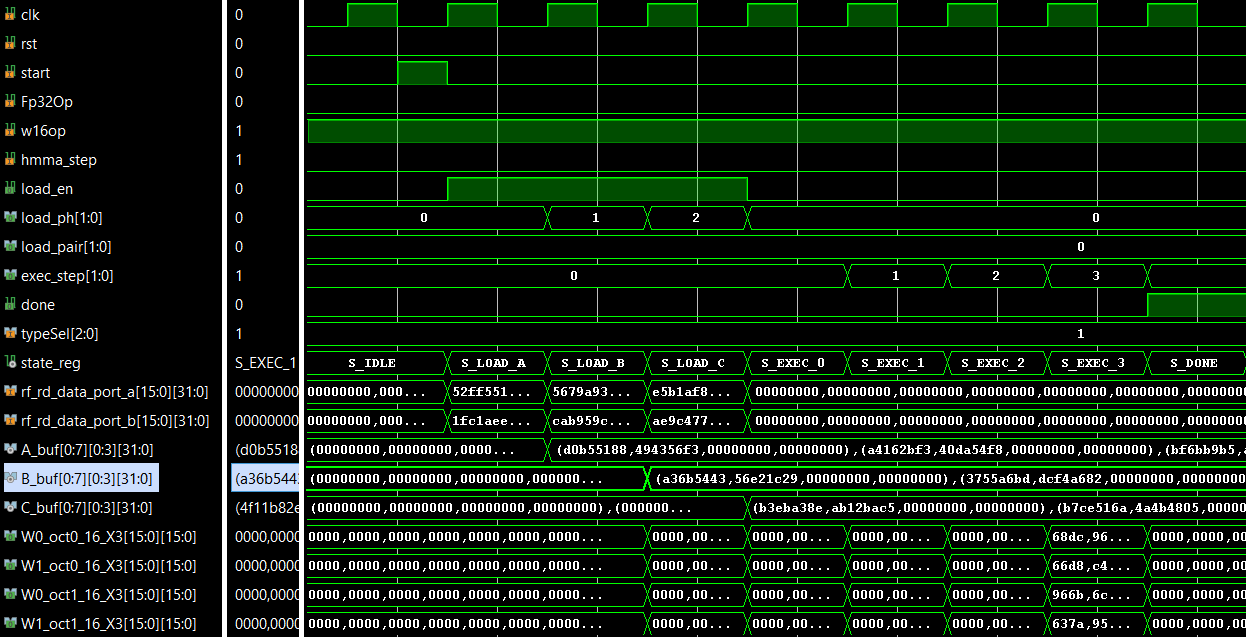
\includegraphics[
    angle=+90,
    width=0.5\textheight
]{Figures/parametricTCUsim.png}
\caption{Standalone RTL simulation waveform of a singular HMMA step 0 instruction in the parametric TCU execution sequence.}
\label{fig:tcu_functional_waveform}
\end{figure}

\newpage
\section{Summary}

This chapter presented in detail the first relase of the parametric TCU architecture. Starting from the concepts introduced related to the granular level parametric DPU introduced in chapter 3, it presented the necessary control and datapath hiererchy needed to implement the parametric higher level accelerator. From a software point of view, it introduced the overall hardware descriptions needed for moving from the singular dot-product operation, to the higher level execution of a matrix multiplication and accumulation operation. 

More in detail, it has been introduced that the higher level wrapper component of the TCU accelerator is split into a FSM and datapath hierechy of design. With the FSM controlling the loading, execution and completion of the singular HMMA related instructions of the sets of the MMA operation, and the datapah organized around two octet cores associated to the 16 threads in total of the SIMD programming model paradigm. Specifically on the datapath, the inner components of the octet core component have been presented : the operand buffers and the DPU array.

Lasty, this chapter presented the functional verification flow that has been done while debugging the components of this first release of the parametric TCU. This debugging has been done through the observation of Vivado waveforms during simulation showing related signals of the components for the related HMMA instructions executed by the testebench of the related formats. 

The next chapters of the thesis will now present the integration step which has been done as soon as the TCU had been varified in its isolated environment. Particularly, chapter 5 will present concepts related to the integration of the TCU component inside a description the Flexgrip plus GPU, and chapter 6 will present the integration of the accelerator with the klessydra T13 RISC-V multi hart core. 